\section{Das Standardmodell}
Das Standardmodell(SM) beschreibt alle bekannten Elementarteilchen und die zwischen ihnen herrschenden Wechselwirkungen. Die Elementarteilchen sind dabei in drei verschiedene Gruppen aufgeteilt: Quarks, Leptonen und Eichbosonen. Quarks und Leptonen sind Fermionen während Eichbosonen offensichtlich Bosonen sind. Die drei grundlegenen Wechselwirkungen, die durch das SM beschrieben werden sind: die elektromagnetische Wechselwirkung, die schwache Wechselwirkung und die starke Wechselwirkung. Die Gravitation wird jedoch nicht durch das SM beschrieben.
Jede Wechselwirkung verfügt über Austauschteilchen. Diese Teilchen sind die zur Kraft gehörenden Eichbosonen. Die Austauschteilchen der starken Wechselwirkung sind die Gluonen, die Austauschteilchen der elektromagnetischen Kraft sind die Photonen und die Austauschteilchen der schwachen Kraft sind die massiven $W^{\pm}$- und $Z^{0}$-Bosonen.
Die Fermionen des Standardmodells werden durch die Wechselwirkungen denen sie unterliegen charakterisiert. Neutrinos, die zu den Leptonen gehören, wechselwirken nur schwach, geladene Leptonen, wie z.B. das Elektron, wechselwirken schwach und elektromagnetisch. Quarks nehmen an jeder Wechselwirkung teil, insbesondere der starken Wechselwirkung\cite{halzen2008quark}.

\section{Quantenchromodynamik}
\subsection{Allgemeines}
Bei der Kollision von Hadronen spielt die Wechselwirkung zwischen Quarks und Gluonen die entscheidende Rolle. Dabei handelt es sich um die starke Wechselwirkung, die Quantenchromodynamik (QCD). Analog zur elektromagnetischen Wechselwirkung wird sie durch eine Ladung bestimmt. Dies ist die Farbladung. Es gibt insgesamt sechs Farben: rot, grün, blau und die dazugehörigen Antifarben. Allerdings können bei geringen Energien nur farbneutrale Teilchen existieren, bei denen sich alle Farben zu weiß addieren. Dies wird als Confinement bezeichnet\cite{halzen2008quark}.

% Die Quantenchromodynamik ist die Theorie, die die starke Wechselwirkung beschreibt. Die Teilchen, die stark wechselwirken sind lediglich Quarks und Gluonen. So wie die elektromagnetische Kraft hat auch die starke Wechselwirkung eine Ladung, welche Farbe genannt wird. Es gibt dabei drei Farben: rot, grün und blau. Zusätzlich existieren noch die dazugehörigen Antifarben. Durch die Quantenchromodynamik wird sowohl die Wechselwirkung zwischen einzelnen Quark in einem Hadron z.B. Proton beschrieben, als auch die Wechselwirkung zwischen Hadronen wie die Wechselwirkungen zwischen Protonen und Neutronen in einem Atomkern.
% \subsection{Regge-Theorie}
% Die Regge-Theorie ist ein Ansatz in der Streutheorie. Dabei werden im Gegensatz zu den ursprünglich zugelassenen ganzzahligen Drehimpulsen in der Partialwellenanalyse komplexe Drehimpulse zugelassen. Daraus ergeben sich sogenannte Trajektorien, die den Drehimpuls durch den Impulsaustausch parametrisieren. Diese Trajektorien bestimmen den Wirkungsquerschnitt der Streuung. Aus experimentellen Ergebnissen ist bekannt, dass dieser mit steigender Energie anwachsen muss. Die Erklärung dafür bildet das Pomeron, ein Austauschteilchen, welches aus mehreren Gluonen besteht. Dieser Glueball trägt dabei zum Anwachsen der starken Kopplungskonstante in Abschnitt \ref{sec:alpha} bei.

\subsection{Die starke Kopplundkonstante $\alpha_s$}\label{sec:alpha}
So wie die elektromagnetische Wechselwirkung, wird auch die Stärke der starken Wechselwirkung durch eine Kopplungskonstante bestimmt. Bei der elektromagnetischen Kraft wird eine theoretisch unendliche Ladung, durch Teilchen-Antiteilchen-Paare, die spontan entstehen und sich wieder vernichten, abgeschirmt. Dies führt zu dem Effekt, dass die Kopplungskonstante $\alpha_{em}$ bei steigenden Energien (d.h. geringerem Abstand zur Ladung) größer wird, weil weniger Abschirmung vorhanden ist\cite{halzen2008quark}. Dasselbe Phänomen gibt es bei der Farbladung. Jedoch wird die Abschirmung durch Quark-Antiquark-Paare von einer Verstärkung der Ladung durch Gluonen übertroffen. Aus diesem Effekt folgt das Confinement und die asympotische Freiheit der Quarks, die besagt dass die Kraft zwischen Quarks bei steigender Energie abnimmt. Auch Hadronisation hängt mit dem Verhalten der starken Wechselwirkung bei unterschiedlichen Energien zusammen.

\subsection{Partonen Verteilungen (PDF)}
Bei der Untersuchung von Hadron-Kollisionen ist es für die theoretische Behandlung nötig die Partonenverteilung innerhalb der Hadronen zu kennen, da diese sich direkt auf die Wirkungsquerschnitte der aller Reaktionen auswirkt. Diese Gerade der Impuls der einzelnen Partonen spielt eine wichtige Rolle. Die Partonverteilungen für Protonen lassen sich Über die Strukturfunktionen der inelastischen Streutheorie herleiten\cite{halzen2008quark}. Sie sind durch Integro-Differential-Gleichungen gegeben und müssen numerisch berechnet werden. 

% Analog zum Formfaktor beim WQS von elastischen Stößen, gibt es bei inelastischen Stößen die sogenannten Strukturfunktionen, aus denen sich der WQS berechnen lässt. Die Strukturfunktionen hängen gleichzeitig von den Matrixelementen der betrachteten Prozesse im Hadron ab. Betrachtet man Gluon-Bremsstrahlung und Paarbildung als Prozesse innerhalb des Hadrons, so lassen sich die Dokshitzer–Gribov–Lipatov–Altarelli–Parisi Gleichungen (DGLAP) aufstellen, die Integro-Differentialgleichungen für die Partonverteilung in Abhängigkeit von dem Impulsübertrag beim inelastischen Stoß und dem Impulsanteil des Partons am Hadron-Impuls darstellen. \comment{Moonstersatz}PDFs finden hauptsächlich in Monte-Carlo-Simulationen Anwendung.

\section{Jet-Physik}
\subsection{Hadronisation}
Bei Kollisionen in Teilchenbeschleunigern wie dem \lhc am \cern, enstehen zunächst freie Quarks. Allerdings sind freie Quarks in der Natur nicht nachzuweisen, da die starke Kopplungskonstante, bei wachsendem Abstand zwischen zwei Teilchen mit Farbladung, wächst. Ein einzelnes Quark hätte demnach ein unendliches Potential. Das Phänomen, dass Quarks nicht einzeln vorkommen wird als \emph{Confinement} bezeichnet. Wenn nun bei einer Reaktion zwei Quarks entstehen, die entgegengesetzte Impulse haben bzw. sich auseinander bewegen, so steigt das Potential zwischen den Quarks an bis genug Energie im Potential ist um ein Quark-Antiquark-Paar zu erzeugen\cite{Artru1983147}. Die beiden entstehenden Quarks bilden nun mit den beiden ursprünglichen Quarks stabile Hadronen. Dieser Prozess wird als Hadronisation bezeichnet. Aus einem einzelnen Quark entstehen dabei eine große Anzahl an Hadronen. Im Detektor werden deshalb Quarks als Hadronenschauer, auch Jets genannt, sichtbar. Beim Detektieren spielt das $b$-Quark eine besondere Rolle, da die Zeit, die das $b$-Quark zur Hadronisation braucht, im Vergleich zu allen anderen Quarks besonders lang ist und deshalb vom $b$-Quark stammende Jets ($b$-Jets) identifiziert werden können.
\subsection{Transversale Masse}
Mit der relativistischen Energie-Impuls-Beziehung lässt sich die Ruhemasse eines Teilchens aus seinem Vierer-Impuls $p^\mu$ berechnen. Auf diese Weise lässt sich aus zwei im Detektor gemessenen Teilchen die Ruhemasse des Mutterteilchens berechnen. So lässt sich zum Beispiel die Ruhemasse des Top-Quarks bestimmen, indem man die Lorentzimpulse der Zerfallsprodukte ($b$-Jet + $W$-Zerfallsprodukte) misst, addiert und die Minkowski-Norm betrachtet. Wenn jedoch Neutrinos eine Rolle spielen, wie in dem Zerfall des $W$-Bosons zu einem geladenen Lepton und einem Neutrino, muss man die Masse über die transversale Masse $M_T$ bestimmen. Dies ist die Masse die sich nur aus den transversalen Impulsen berechnet. Das Maximum der transversalen Masse ist dann die Ruhemasse des Mutterteilchens. Dies findet Anwendung in Messungen der $W$-Masse.
\section{Top-Quark Physik}
\section{Vorhersage des Top-Quarks}
Die Existenz des Top-Quarks wurde vorhergesagt um die Brechung der $CP$-Symmetrie zu erklären. Hiernach ist eine Brechung dieser nur möglich, wenn in den Matrixelementen eine komplexe Phase auftaucht. Dafür ist es notwendig, dass die Dimension der CKM-Matrix, die einen Faktor im Matrixelement beschreibt, mindestens drei beträgt. Daher muss mindestens eine dritte Generation von Quarks existieren\cite{KOBAYASHI1989199}. 
% Aus Experimenten mit Kaonen wurde deutlich, dass die $CP$-Symmetrie verletzt ist. Die Eigenzustände eines Kaons zur $CP$-Symmetrie können als Superpositionen von Kaon und Antikaon beschrieben werden. Beide Zustände zerfallen in Pionen, wobei die Masse des Kaons nur geringfügig größer ist als die Masse von drei Pionen. Nun haben zwei Pionen einen $CP$-Eigenwert von $+1$ während eine ungerade Anzahl von Pionen einen Wert von $-1$ hat. Daraus folgt, dass das Kaon mit $CP=1$ schnell in zwei Pionen zerfällt, während das andere Kaon langsam in drei Pionen zerfällt. Im Experiment wurde nachgewiesen, dass selbst nach einer Zeit in der die kurzlebigen Kaonen zerfallen sein müssen, noch immer Kaonen in zwei Pionen zerfallen. Dies stellt eine Verletzung der $CP$-Symmetrie dar. Um diese $CP$-Brechung zu erklären muss eine komplexe Phase in die Elemente der CKM-Matrix eingeführt werden. Dies ist jedoch nur möglich wenn die Matrix mindestens eine Größe von $3\times 3$ hat. Deswegen ist eine dritte Generation von Quarks notwendig.
 
\section{Produktion von Top-Quarks}
Die Entstehung von Top-Quarks ist abhängig von den kollidierenden Teilchen und der Schwerpunktsenergie der Kollision. Bei Elektron-Positron-Kollisionen wie am \lep würden Top-Quark-Paare hauptsächlich durch Annihilation zu einem Photon oder $Z^0$-Boson entstehen. Am \lep geschah dies jedoch aufgrund zu geringer Schwerpunktsenergie nicht. Am \tevatron war der vorherrschende Produktionsprozess die Annihilation von zwei leichten Quarks. Der Grund dafür ist, dass bei der Schwerpunktsenergie des \tevatron\ s die ursprünglichen Konstituenten der Protonen und Antiprotonen im Gegensatz zu den See-Quarks und Gluonen eine große Rolle spielen. Bei hoher Schwerpunktsenergie dominiert die Produktion über Gluonen wie in Abb. \subref{fig:ttbar_prod_feyn_gg1}-\subref{fig:ttbar_prod_feyn_gg3} zu sehen\cite{Lemmer:2014zua}. Der Grund dafür liegt in der Energieabhängigkeit der PDF. Diese Prozesse finden am \lhc statt. Der Zerfall eines Top-Quarks findet in nahezu jedem Fall über die schwache Wechselwirkung zu einem $b$-Quark statt.


% Die Produktion von Top-Quarks am \lep am \cern würde vorherrschend über Annihilation der Elektronen geschehen. Diese Annihilation kann über Photon oder $Z$-Boson stattfinden. Es ist in erster Ordnung nur möglich Top-Paare zu erzeugen, weswegen eine besonders hohe Schwerpunktsenergie notwendig wäre. Es wären ca. $340$~GeV nötig gewesen während die Höchstleistung des LEP bei $209$~GeV lag. Am \tevatron wurden hauptsächlich Top-Paare durch Annihilation zweier leichter Quarks erzeugt. Aufgrund der geringen Energie ($2$~TeV) rühren der Großteil der Reaktionen von Quark-Quark-Interaktionen her. Wechselwirkungen zwischen Gluonen spielen eine untergeordnete Rolle. Die Produktion von einzelnen Top-Quarks kann nur über die schwache Wechselwirkung stattfinden. Dazu muss allerings die Quark-Generation gewechselt werden, weswegen diese Reaktion unterdrückt ist. Am \lhc werden Top-Quarks vor allem über Gluon-Gluon-Wechselwirkungen erzeugt. In Abbildung \ref{fig:ttbar_prod_feyn} sind die Feynmandiagramme der wichtigsten Produktionsprozesse dargestellt. 
% Aufgrund seiner geringen Lebensdauer zerfällt das Top-Quark bevor es hadronisiert. Die Wahrscheinlichkeit für einen Zerfall über ein $W$-Boson in ein $b$-Quark ist nahezu $100\%$.
\begin{figure}
	\centering
			\subfigure[]{
		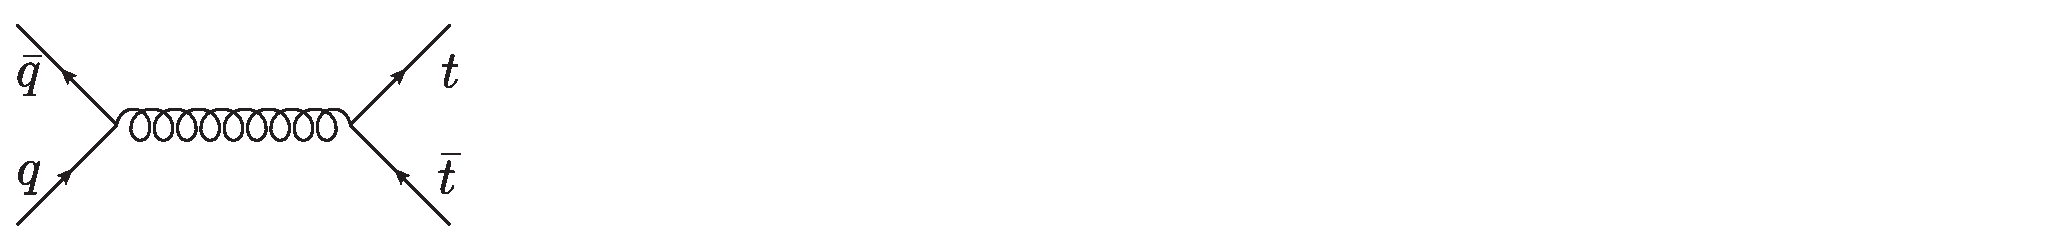
\includegraphics[width=0.4\textwidth]{input/ttbar_prod_feyn_qq.pdf}
			\label{fig:ttbar_prod_feyn_qq}
		}
					\subfigure[]{
		
\includegraphics[width=0.4\textwidth]{input/ttbar_prod_feyn_gg1.pdf}
			\label{fig:ttbar_prod_feyn_gg1}
		}\\
	\subfigure[]{
		
\includegraphics[width=0.4\textwidth]{input/ttbar_prod_feyn_gg2.pdf}
			\label{fig:ttbar_prod_feyn_gg2}
		}
			\subfigure[]{
		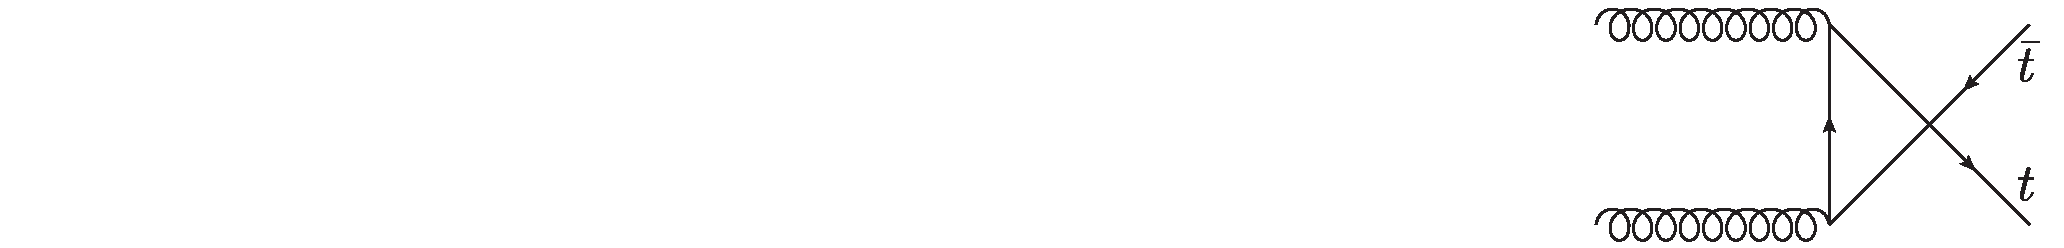
\includegraphics[width=0.4\textwidth]{input/ttbar_prod_feyn_gg3.pdf}
			\label{fig:ttbar_prod_feyn_gg3}
		}
		\caption{\ttbar\ Erzeugung über die starke Wechselwirkung. \subref{fig:ttbar_prod_feyn_qq} Annihilation (vorherrschend bei Proton-Antiproton-Kollisionen bei geringen Energien ), \subref{fig:ttbar_prod_feyn_gg1}-\subref{fig:ttbar_prod_feyn_gg3} über Gluonen (vorherrschend bei Hadron-Hadron-Kollisionen bei großen Energien)\cite{Lemmer:2014zua}. }
\label{fig:ttbar_prod_feyn}
\end{figure}


\section{Entdeckung und Eigenschaften}
\comment{Quellen sind vor allem PDG}Das Topquark wurde erstmals 1995 am \tevatron in den Detektoren \dzero und \cdf nachgewiesen\cite{PhysRevLett.74.2626}. Mit einer Ruhemasse von $173.34 \pm 0.27(\text{stat.}) \pm 0.71 (\text{sys.})$~GeV ist es das schwerste Elementarteilchen \cite{ATLAS:2014wva}. Seine Zerfallsbreite ist $2.0\pm0.5$~GeV und seine Lebensdauer ist damit ca. $5\cdot10^{-25}$~s (berechnet aus \cite{2006EPJC...48..835Q}). Diese geringe Lebensdauer liegt deutlich unter der Zeit die das Top-Quark zur Hadronisation brauchen würde. Damit ist es das einzige Quark, das zerfällt bevor es Hadronisieren kann. Dies macht es besonders leicht die Masse des Top-Quarks über seine Zerfallsprodukte zu bestimmen.
 

\section{Higgs-Boson Physik}
\subsection{Der Higgs-Mechanismus}
Das Higgs-Boson ist das neuste Teilchen des Standardmodells. Es wurde 1964 von Peter Higgs \emph{et al.} zusammen mit dem Higgs-Mechanismus postuliert\cite{Higgs:1964pj}. Der Higgs-Mechanismus erklärt, warum $W^\pm$- und $Z^0$-Bosonen im Gegensatz zu Photonen und Gluonen eine Ruhemasse besitzen. Nach der allgemeinen Eichtheorie können Austauschbosonen keine Masse haben. Um dies zu erklären führten Higgs \emph{et al.} das Weak-Symmetry-Breaking ein, nach welchem das Potential im Lagrangian über zwei Minima verfügt. Wenn man nun das Potential um eines der Minima entwickelt, so tauchen durch die Entwicklung neue Felder auf von denen eines das Higgs-Feld darstellt\cite{halzen2008quark}. Das andere Feld spiegelt sich nur als komplexe Phase wieder und kann aufgrund der lokalen Eichinvarianz absorbiert werden. Die Existenz eines Higgs-Feldes suggeriert die Existenz eines massiven neutralen skalaren Bosons, welches Higgs-Boson genannt wird.
Über die sogenannte Yukawa-Kopplung koppelt das Higgs-Boson auch an Fermionen, und erzeugt auch deren Masse.
\subsection{Entdeckung}
Im Jahr 2012 wurde am \lhc in Genf ein neutrales Skalarboson mit einer Masse von $125.36 \pm 0.37(\text{stat.}) \pm 0.18 (\text{syst.})$~GeVentdeckt \cite{Aad:2012tfa}. Damit stimmt es in seinen Eigenschaften mit dem gesuchten Higgs-Boson überein. Es wurde zunächst über die Zerfallskanäle $H \rightarrow 4 \ell$, $H \rightarrow \gamma\gamma$, $H \rightarrow e\nu\mu\nu$ und Zerfallskanäle zu $ZZ^*$, $WW^*$, $\tau^+\tau^-$ und $\bbbar$ gemessen. In Abb. \ref{fig:higgsdiscovery} sind Ergebnisse der Suche nach dem Higgs-Boson aus den kombinierten Daten für eine Schwerpunktsenergie von $\sqrt{7}$ und $\sqrt{8}$~TeV~zu sehen.
\begin{figure}
\centering
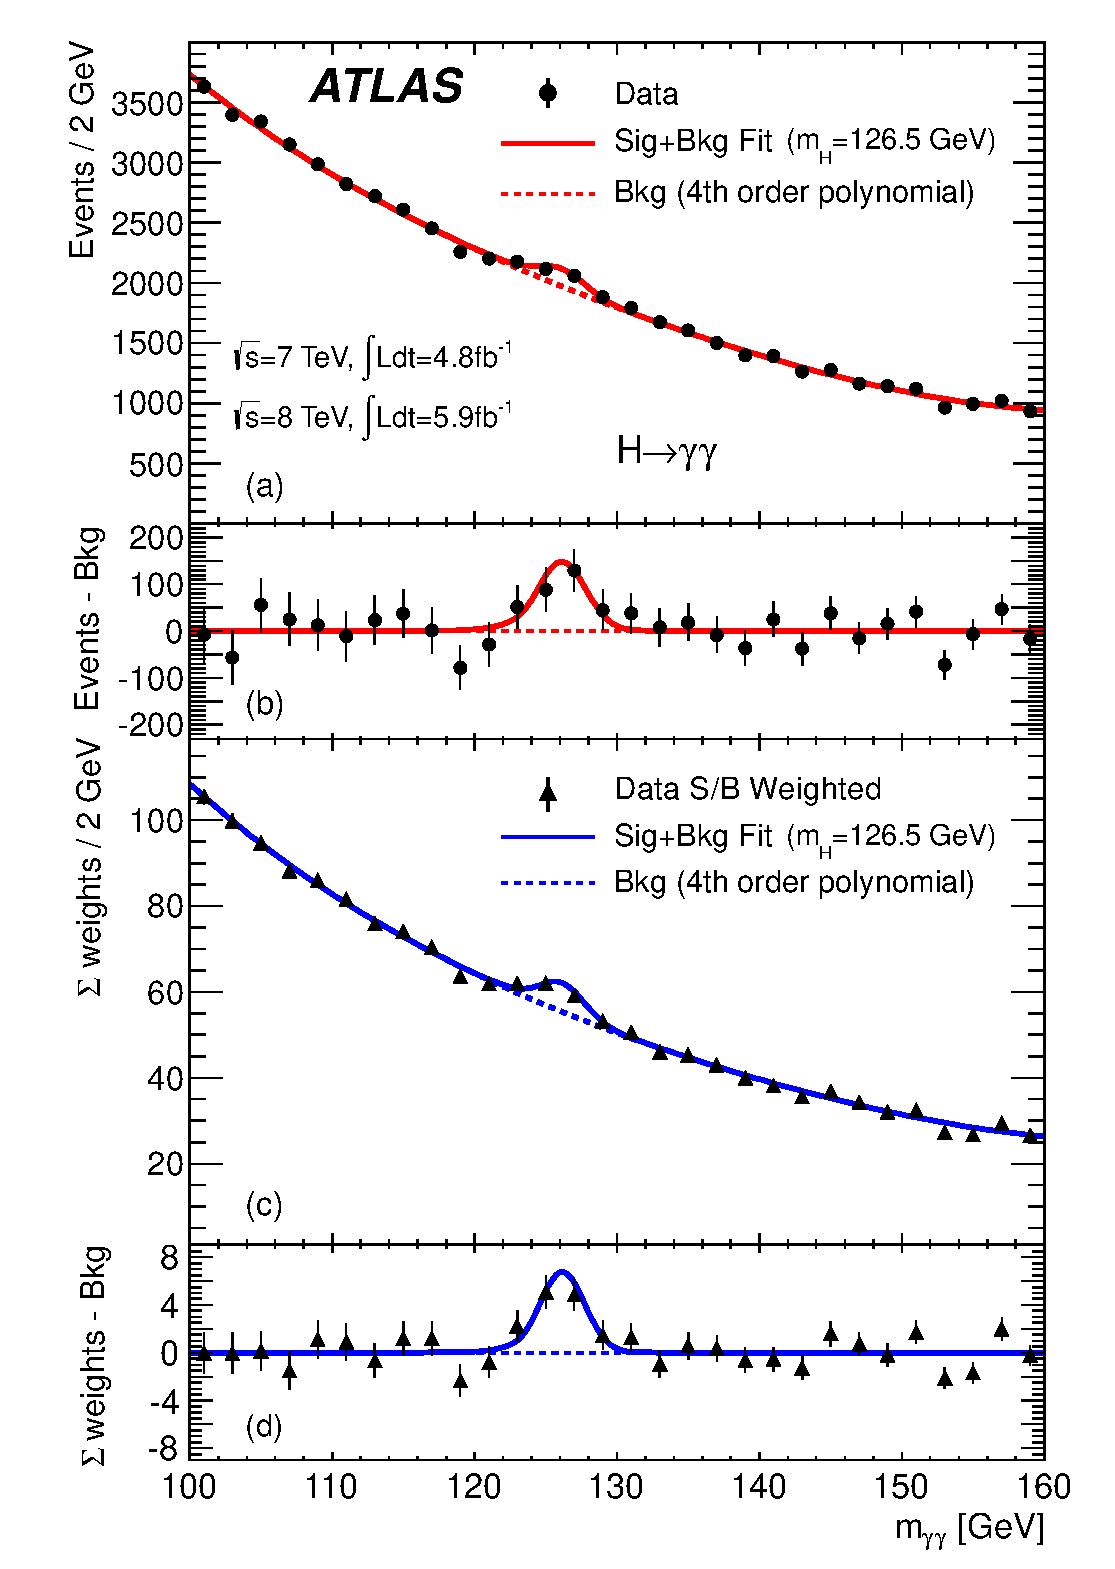
\includegraphics[scale = 0.5]{input/mggweighted_panel_nonorm.eps}\caption{Ergebnisse der Suche nach dem Higgs-Boson aus \cite{Aad:2012tfa} in dem $H \rightarrow \gamma\gamma$-Kanal. Es ist Anzahl der Ereignisse in Abhängigkeit von der invarianten Masse der entstehenden Photonen dargestellt. Gemessene Daten sind durch Punkte gekennzeichnet. Die gestrichelte Linie zeigt den aus Simulationen entnommenen Hintergrund. Die durchgezogenen Linien sind ein Fit für erwartete Hintergund-Ereignisse zusammen mit durch ein 126.5~GeV schweres Higgs-Boson erzeugte Ereignisse. Die beiden schmalen Plots zeigen die Anzahl der Ereignisse nachdem der Hintergrund von den Messungen abgezogen wurde. Die zweite Hälfte des Plots zeigt die Daten nachdem die Ereignisse gewichtet wurden.}\label{fig:higgsdiscovery}
\end{figure}

